
%\documentclass[submit,techrep]{ipsj}
%\documentclass{ipsj}
\documentclass[submit,techrep]{ipsj}

\usepackage[dvips]{graphicx}
\usepackage{latexsym}
\usepackage{algorithm}
\usepackage{algorithmic}
\usepackage{amsmath}

\bibliographystyle{ipsjunsrt}

\def\Underline{\setbox0\hbox\bgroup\let\\\endUnderline}
\def\endUnderline{\vphantom{y}\egroup\smash{\underline{\box0}}\\}
\def\|{\verb|}


\setcounter{巻数}{57}
%\setcounter{号数}{1}
%\setcounter{page}{1}


%\受付{2016}{6}{30}
%\再受付{2015}{7}{16}   %省略可能
%\再再受付{2015}{7}{20} %省略可能
%\採録{2016}{7}{1}




\begin{document}


\title{湯気のビジュアルシミュレーション}

\etitle{Visual Simulation of Steam}

\affiliate{OUJ}{放送大学\\
The Open University of Japan}


%\paffiliate{JU}{情報処理大学\\
%Johoshori University}

\author{佐野 宏行}{Hiroyuki Sano}{OUJ}
\author{浅井 紀久夫}{Kikuo Asai}{OUJ}

\begin{abstract}
本研究ではCGによる湯気のビジュアルシミュレーションを行った.湯気の発生と消滅のプロセスからCGによるシミュレーションに必要なモデルを構築し,水蒸気量と温度のパラメータにより実用的な計算時間でアニメーションの生成を可能とする.流体計算は格子法と粒子法を組み合わせることにより相転移を行い,湯気の微細な動きを再現する手法を提案する.
\end{abstract}


\begin{jkeyword}
ビジュアルシミュレーション,湯気,流体現象
\end{jkeyword}

\maketitle

%1
\section{はじめに}

コンピュータグラフィックス(CG)において湯気の表現は現実感を増幅する場合に非常に重要な要素である.
CGの研究においては水,煙といった流体シミュレーションの研究は盛んに行われるが,水の特徴である三態変化を扱う研究はほどんど行われていない.
特に水が相転移する際に発生する湯気の表現手法は確立しておらず,クリエーターによる熟練した技術と経験が必要となっている.
また近年普及が期待されるVR,AR技術においても現実感を向上させるための手段として湯気は重要な要素となる.

本研究においては湯気の発生,消滅のプロセスに基づいてCGにおける湯気のモデルを構築し,
温度,水蒸気量といった湯気の状態に影響するパラメータを変化させることによる湯気の可視化を行う.
流体計算は格子法と粒子法を組み合わせる手法を提案し,水滴の湯気と水蒸気の間の相転移を本手法へ適用し,湯気の微細な動きを再現する手法を提案する.


%なお本研究では常温の空気中に存在する沸騰の状態ではない液体の水から湯気が発生している状態を対象とする.
%これにより従来のCGでは作成できない温度,水蒸気量を考慮した温泉,暖かい料理といったシーンを表現可能となり,よりCGの表現能力を上げることができる.VR,AR技術においても現実感を増幅するための要素として応用が期待できる.

%\footnotetext{本文は実際には論文誌ジャーナル編集委員会で作成したものである.}

%2
\section{既存研究}

湯気の発生に関する表現に特化したCGによる流体シミュレーションの研究は行われていない.
湯気に近い表現としては煙\cite{Fedkiw2001},雲\cite{Dobashi2000}\cite{Miyazaki2001}\cite{Miyazaki2002},火山噴煙\cite{Mizuno2003}\cite{Mizuno2004},水煙\cite{Nielsen2013},水滴と水泡\cite{Mihalef2009}のシミュレーションの研究がある.
水の蒸発,凝固,凝結といった性質を包括的に扱う研究\cite{Fujisawa2008}はあるが湯気に関しては考慮されない.
\cite{Foster1997}では湯気(Steam)の表現の言及はあるが水蒸気量を考慮した表現は行われていない.
流体力学では複数の相が混じり合う物質は混相流(multi phase flow),湯気のように気体と液体が混合する物体の動きは気液二相流として研究が行われているがCGの作成を目的とはしていない.

湯気の表現に必要な水の液体と気体間の相転移,温度の熱拡散,蒸気の分子拡散をCGに適用した研究がある.
水の液体と気体間の相転移のモデルは宮崎ら\cite{Miyazaki2001}\cite{Miyazaki2002}により飽和水蒸気量を利用するモデルが提案された.
温度の熱拡散のモデルはFosterら\cite{Foster1997},宮崎ら\cite{Miyazaki2002},蒸気の分子拡散のモデルは宮崎ら\cite{Miyazaki2002}によりCGに適用された.

本研究では湯気の流体現象の計算に粒子法と格子法の両方を用いるFLIP法をベースとした手法を採用する.
CGにおいて粒子法と格子法を組み合わせることによる手法は雨氷\cite{Ishikawa2015},雪\cite{Stomakhin2013}の表現において適用される.

\section{提案法}
本論文では湯気のシミュレーションと可視化を実際の湯気の発生と消滅のプロセスをもとに格子法と粒子法を用いた手法を提案する.
流体の空気と水蒸気の気体部分は格子法,湯気の水滴部分は粒子法によって表現を行い,
流体との相対速度から発生する抗力を考慮した湯気の動きを再現する.
流体のモデルはFedkiwら\cite{Fedkiw2001}の手法に基づき非粘性,非圧縮の流体を仮定する.
熱,水蒸気の発生と移動は熱拡散と分子拡散,流体の速度による自然対流による移動の双方を考慮する.
水滴から水蒸気の間の相転移は宮崎ら\cite{Miyazaki2001}\cite{Miyazaki2002}による飽和水蒸気量を利用するモデルを格子法と粒子法を用いる手法へ適用する.

\section{湯気のシミュレーション}
\subsection{湯気の発生と消滅のプロセス}
\begin{figure}[h]
\centering
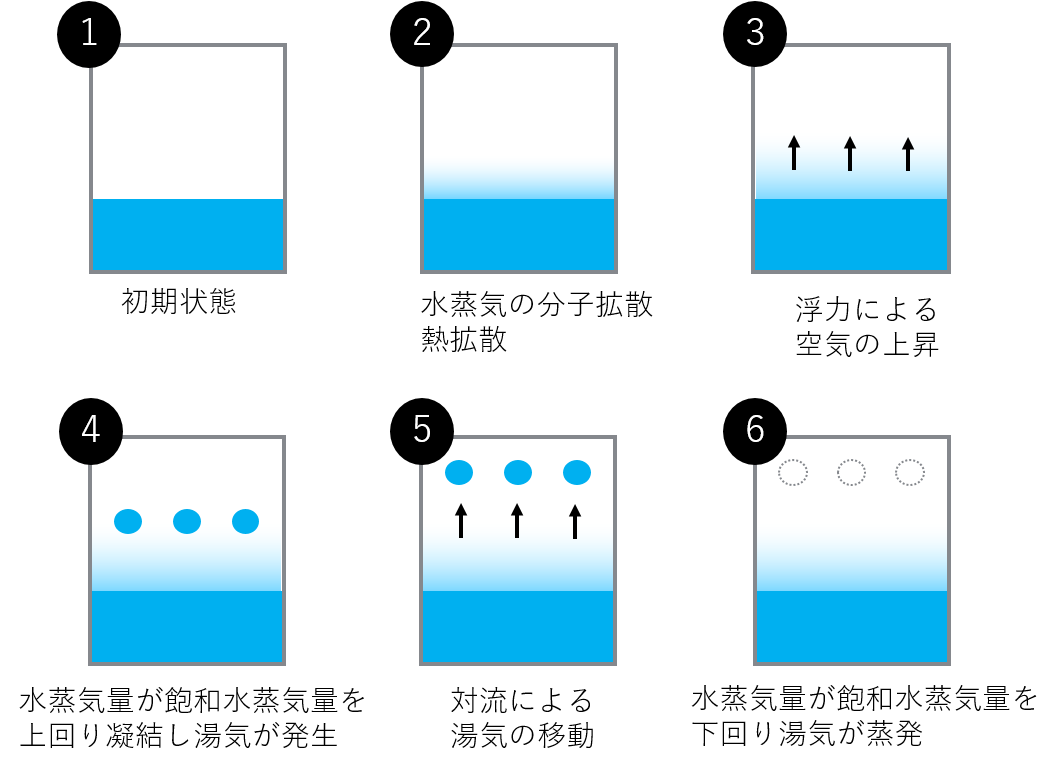
\includegraphics[width=0.8\linewidth]{process.eps}
\caption{湯気の発生と消滅のプロセス}
\label{process}
\end{figure}
湯気が発生してから消滅するまでのプロセスを図(\ref{process})に記載する.	
初期状態としては常温の空気内に沸騰状態ではないが空気より高い温度の水があると仮定する.
水は水面上から蒸発し,蒸発した水蒸気は分子拡散により周囲へ拡散する.
同時に水の温度は空気よりも高いため温度勾配により熱拡散が起こり熱が水から空気へ移動する.
空気の温度が上昇すると空気の密度が周囲の空気より低くなることにより浮力が発生する.
浮力により空気に上方向の力が働き,対流が発生する.
この対流により空気に含まれる水蒸気,熱が移動する.
空気中に含まれる水蒸気量が飽和水蒸気量を超えた場合に凝結することで水滴が発生する.
凝結は大気中の細かい塵を核として行われる.
この水滴の粒子に対して光が当たった際に散乱が起こり白く見えることで湯気として認識される.
凝結により発生する水滴の粒子は光の波長と同程度,もしくは少し大きめの大きさとなりミー散乱という現象が発生する.
ミー散乱は粒子のサイズが大きくなるにつれて前方の指向性が高くなり側方,後方への散乱は弱くなる.
空気中に含まれる水蒸気量が飽和水蒸気量を下回った場合,水滴が空気中に蒸発し湯気が消滅する.

\subsection{シミュレーションモデル}

流体の速度$\upsilon=(u,v,w)$は非粘性,非圧縮のオイラーの運動方程式(\ref{continuity},\ref{euler})によって与えられる.

\begin{equation}
\label{continuity}
\nabla \cdot \upsilon = 0
\end{equation}
  \begin{equation}
  \label{euler}
  \frac{\partial \upsilon}{\partial t} = -(\upsilon \cdot \nabla)\upsilon - \nabla p + B + f
  \end{equation}

$p$は圧力,$B$は浮力,$f$は風などによる外力を表す.浮力$B$はブシネスク近似より式(\ref{buoyancy})で定義する.
\begin{equation}
\label{buoyancy}
B=k_{b}\frac{T-T_{a}}{T_{a}}z
\end{equation}
$k_{b}$は浮力の係数,$T$は流体の温度,$T_{a}$は環境温度,$z$は上方向のベクトルである.

湯気の密度$q_{c}$と水蒸気$q_{v}$の密度は次式で定義する.
\begin{equation}
\label{steam}
\frac{\partial q_{c}}{\partial t} = -(\upsilon \cdot \nabla)q_{c} + C_{s}
\end{equation}
\begin{equation}
\label{vapor}
\frac{\partial q_{v}}{\partial t} = -(\upsilon \cdot \nabla)q_{v} + D_{v}\nabla^2q_{v} - C_{s} + S_{v}
\end{equation}
$D_{v}$は水蒸気の分子拡散係数,$C_{s}$は相転移によって発生する湯気の量,$S_{v}$は水蒸気源から水蒸気の供給量である.

温度$T$は次式で表される.
\begin{equation}
\label{temperature}
\frac{\partial T}{\partial t} = - (\upsilon \cdot \nabla)T + D_{t}\nabla^2T +  QC_{s} + S_{T}
\end{equation}
ここで$D_{t}$は熱拡散率,$Q$は潜熱係数を表す.
右辺第一項は熱対流,第二項は熱拡散,第三項は相転移による潜熱,第四項は外部の熱源からの熱量を表す.

分子拡散係数$D_{v}$は次式で表される.これはアインシュタイン・ストークスの式より温度に依存する.
\begin{equation}
\label{diffusion}
D_{v}=D_{0}T
\end{equation}
ここで$D_{0}$は分子拡散係数を決定するためのパラメータである.

相転移によって増減する湯気の量$C_{s}$は次式で表される.
\begin{equation}
\label{transition} 
C_{s} =
\begin{cases}
 \alpha(q_{v}-q_{s}) & q_{v} \geq q_{s}\\
 \max\left(\alpha(q_{v}-q_{s}),-q_{c}\right) & q_{v} < q_{s}
\end{cases}
\end{equation}
\begin{equation}
\label{saturation}
q_{s} = \min\left(S_{a} \exp\left(\frac{-S_{b}}{T+S_{s}}\right),q_{v}+q_{c}\right)
\end{equation}
ここで$\alpha$は相転移率である.
$q_{s}$の$\min$関数の第一引数は飽和水蒸気密度を表し
$S_{a},S_{b},S_{s}$は飽和水蒸気密度を決定するためのパラメータである.
$q_{s}$の$\min$関数の第二引数で湯気と水蒸気の密度の合計値を指定する.
これにより水蒸気と湯気の密度の合計値が飽和水蒸気密度を超えている場合にも湯気の消滅を行う.
湯気の消滅は湯気の密度以上行うことはない.

湯気の速度$\upsilon_{s}$は流体との相対速度から発生する抗力,重力を考慮して次式で表される.
\begin{equation}
\label{lagurange}
\frac{d\upsilon_{s}}{dt} = - F_{drag} + mg
\end{equation}
\begin{equation}
\label{dragforce}
F_{drag} = - C_{D} (\upsilon_{s} - \upsilon)^\beta
\end{equation}
$F_{drag}$は抗力,$C_{D}$は抗力を決定するためのパラメータ,$\beta$はレイノルズ数を表しこれは粒子の半径に依存する.

\begin{figure*}[th]
\centering
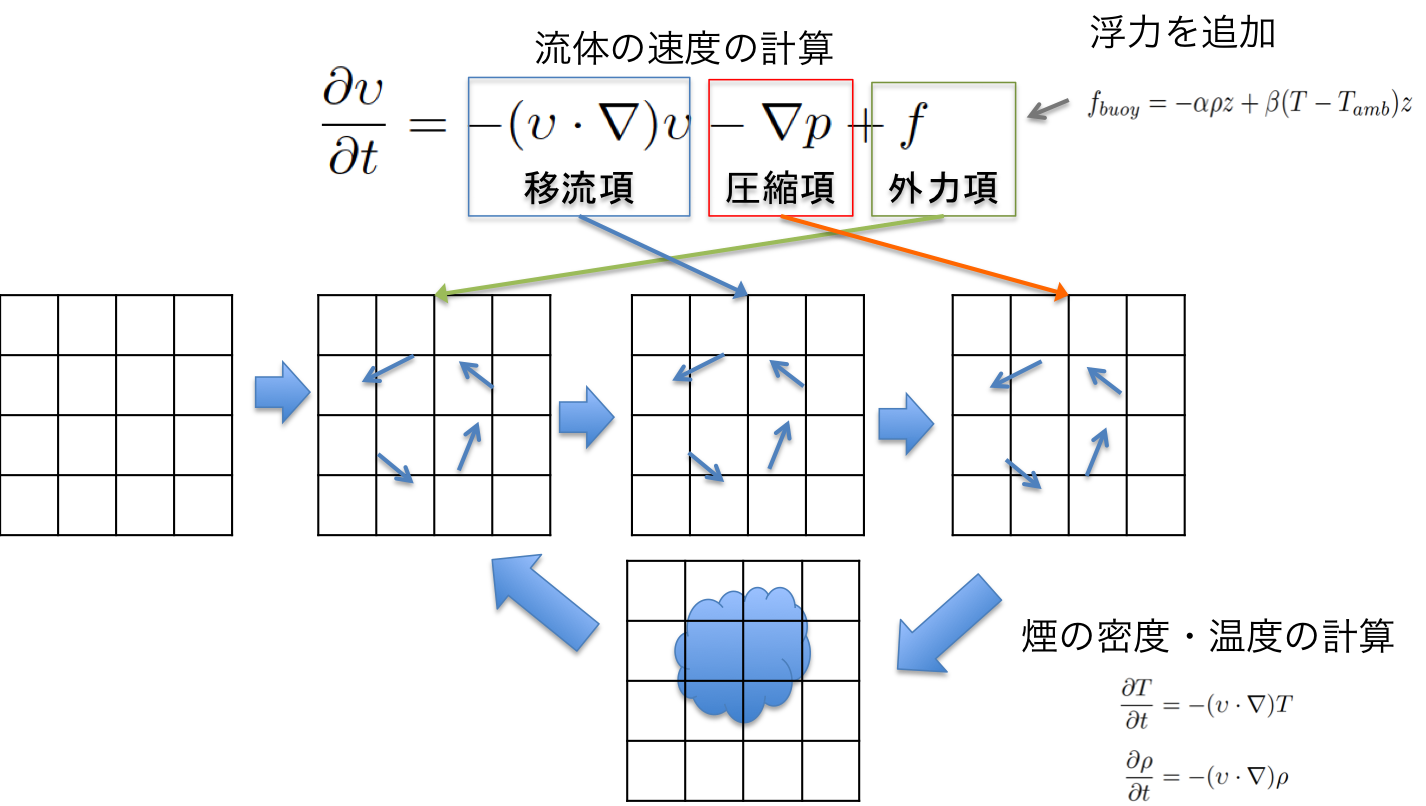
\includegraphics[width=0.8\linewidth]{overview.eps}
\caption{提案法の概要}
\label{overview}
\end{figure*}
\subsection{実装}

\begin{figure}[bh]
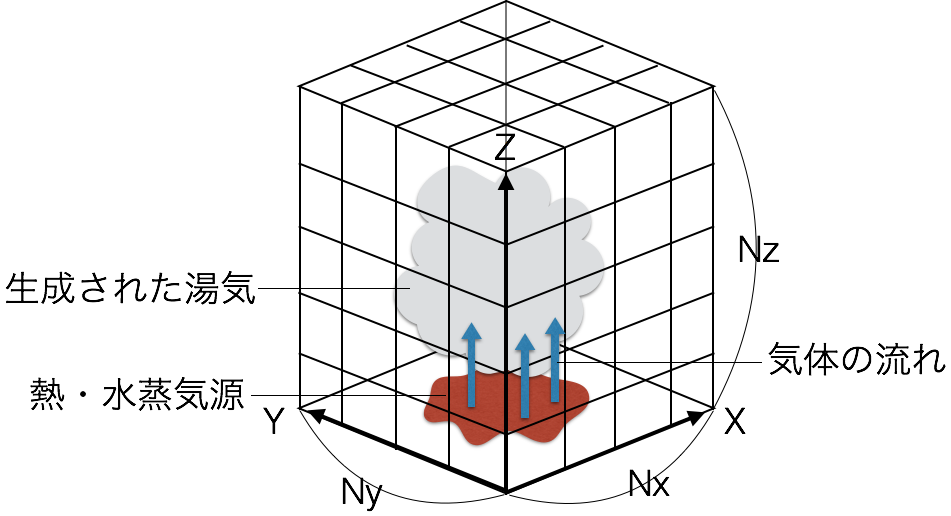
\includegraphics[width=0.7\linewidth]{simulation.eps}
\caption{湯気のシミュレーション空間}
\label{simulation}
\end{figure}



シミュレーション空間は$N_{x} \times N_{y} \times N_{z}$の格子に分割し各格子点に温度$T$,水蒸気の密度$q_{v}$,流体の速度$\upsilon$を割り付ける.格子には温度,水蒸気の密度を格子の面に定義するスタガード格子を採用する.
初期状態として水蒸気源と熱源が存在する部分には水蒸気密度と温度の固定値を割り付ける.
水蒸気源と熱源は空間の底面から発生し,発生量の分布はユーザにより定義する.
湯気は粒子により表現し粒子には格子空間上の位置,速度,質量が格納される.
粒子は質量が一定で粒子同士の衝突,粒子から格子の流体の速度,温度に対する影響はないと仮定する.

図\ref{overview}に本シミュレーション空間上での1タイムステップ中の処理の流れを示す.

\begin{enumerate}
\item {\bf 粒子を格子の値へ変換.}格子内の湯気の粒子の質量を合計し,すべての格子に対して湯気の密度$q_{c}$を計算する.
\item {\bf 相転移による粒子,格子の値の追加,削除.}式(\ref{transition})の相転移のモデルを用いて相転移によって増減する湯気の量$C_{s}$を求め,湯気と水蒸気量の追加,削除を行う.
$C_{s} \geq 0$の場合,格子内に湯気の粒子を追加する.
湯気の粒子の位置は格子内のランダムの位置とし,速度は粒子の位置にある速度を格子面に定義される速度から線形補間により求め,質量は一定とする.
これを追加した粒子の質量の合計が$C_{s}$になるまで処理を続ける.
$C_{s} < 0$の場合,格子内の湯気の粒子の質量を削除する.
これを削除した粒子の質量の合計が$C_{s}$になるまで処理する.
湯気の粒子の追加と削除もしくは処理の後,温度へ$C_{s}$に依存した潜熱の追加,水蒸気の密度$q_{v}$から$C_{s}$の減算,質量が0の湯気の粒子の削除処理を行う.
\item {\bf 格子の速度計算.}非粘性,非圧縮のオイラーの運動方程式(\ref{continuity},\ref{euler})をFedkiwら\cite{Fedkiw2001}の手法に基づき外力,浮力,圧力,移流により流体の速度を計算する.
\item {\bf 格子の値更新.}温度と水蒸気量を式(\ref{temperature},\ref{vapor})に基づき計算する.式(\ref{temperature},\ref{vapor})は共に第一項が対流項,第二項が拡散項となる.
対流項はセミラグランジュ法,拡散項は拡散方程式の数値解析を用いる.拡散項の数値解法で本研究で採用した陽解法の場合はCFL条件によりタイムステップ幅に厳しい制限を課す必要がある.
\item {\bf 粒子の速度計算.}粒子の速度を式(\ref{lagurange})に基づき計算する.抗力$F_{drag}$は格子と粒子の速度の間の相対速度により求める.この計算で用いる格子の速度は粒子の位置にある速度を格子面に定義される速度から線形補間により求める.
\item {\bf 粒子の位置更新.}粒子の位置を粒子自体の速度を追加することにより求める.
\end{enumerate}

\begin{figure*}[t]
  \begin{center}
    \begin{tabular}{c}

      % 1
      \begin{minipage}{0.25\hsize}
        \begin{center}
          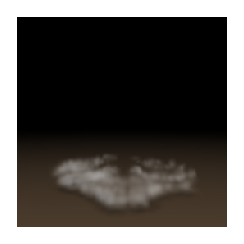
\includegraphics[clip, width=4cm]{./render_20.eps}
          \hspace{1.6cm} (1)20タイムステップ後
        \end{center}
      \end{minipage}

      % 2
      \begin{minipage}{0.25\hsize}
        \begin{center}
          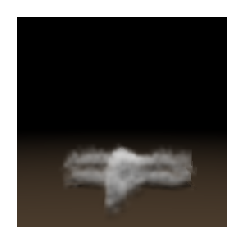
\includegraphics[clip, width=4cm]{./render_40.eps}
          \hspace{1.6cm} (2)40タイムステップ後
        \end{center}
      \end{minipage}

      % 3
      \begin{minipage}{0.25\hsize}
        \begin{center}
          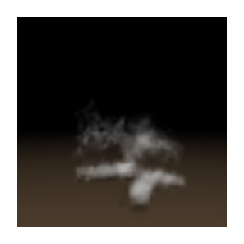
\includegraphics[clip, width=4cm]{./render_60.eps}
          \hspace{1.6cm} (3)60タイムステップ後
        \end{center}
      \end{minipage}

      % 4
      \begin{minipage}{0.25\hsize}
        \begin{center}
          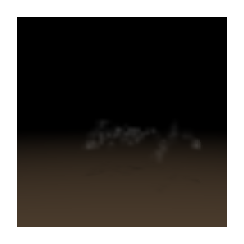
\includegraphics[clip, width=4cm]{./render_80.eps}
          \hspace{1.6cm}  (4)80タイムステップ後 
        \end{center}
      \end{minipage}  

    \end{tabular}
    \caption{湯気のシミュレーションのレンダリング結果}
    \label{result}
  \end{center}
\end{figure*}

\section{結果}

湯気のシミュレーションのレンダリング結果を図(\ref{result})に示す.
格子法と粒子法を用いることで,格子法のみでは実現が困難な水滴の発生位置による微細な湯気の動きを再現した.
本レンダリング結果では湯気の発生分布が大きく2つに分かれている様子を確認した.
レンダリングは格子ごとに湯気の密度を合計し,ボリュームレイキャスティング法により行った.
シミュレーション空間は32×32×32の格子で,シミュレーションで発生した粒子数は3,000個から4,000個となった.
計算時間はIntel Core i5-6200U 2.3GHzのCPUを用いて1タイムステップあたり3秒から4秒となった.

\section{まとめ}
本研究では湯気の発生と消滅のプロセスからシミュレーションモデルを構築し,格子法と粒子法を組み合わせることにより湯気の微細な動きを再現した.
課題としてはパラメータによる調整が困難であることがあげられる.本来の物理モデルより最適なパラメータを決定し,ユーザによる編集を可能とする手法を考案することにより解決できると考えられる.
今後の発展としては粒子として表現した水滴を直接レンダリングすることにより,さらに現実感のあるレンダリング,GPUによるリアルタイムの計算を行うことが考えられる.

\bibliography{onsen}

\end{document}
